\documentclass[a4paper,11pt,exos]{nsi} % COMPILE WITH DRAFT


\pagestyle{empty}
\begin{document}

%Exercice 1E12


%\subsection*{NOM, Prénom : \dotfill} 

\classe{\premiere spé}
\titre{Ceinture marron 02 - Corrigé}
\maketitle\

\begin{exercice}[ : Trouver l'équation d'une parabole]
    Quelle est l'expression de la fonction polynomiale $f$ du second degré qui passe par les points de coordonnées $(-3;4)$, $(0;-5)$ et $(3;22)$ ?\\
    Donner la forme développée de $f$.

    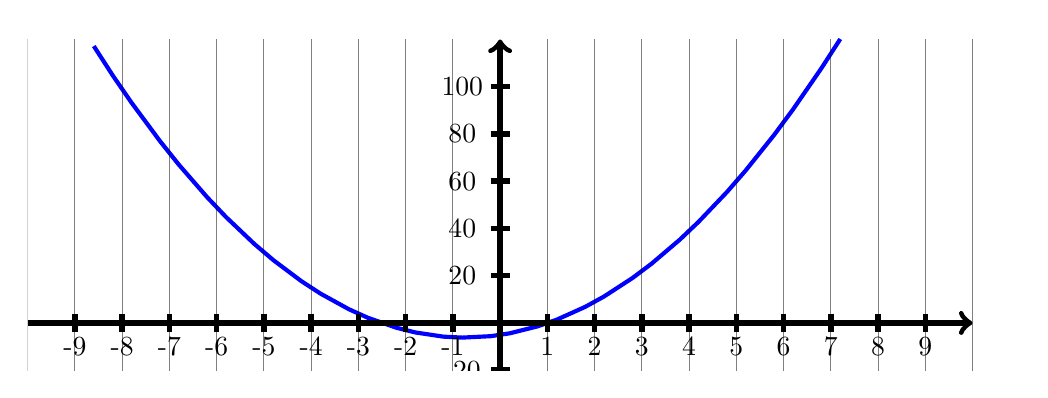
\begin{tikzpicture}[baseline,scale = 0.6]

        \tikzset{
          point/.style={
            thick,
            draw,
            cross out,
            inner sep=0pt,
            minimum width=5pt,
            minimum height=5pt,
          },
        }
        \clip (-10,-1) rectangle (11,6.25);
            
        \draw[color={blue},line width = 1.5] ;
        \draw[color={blue},line width = 1.5] ;
        \draw[color={blue},line width = 1.5] ;
        \draw[color={blue},line width = 1.5] ;
        \draw[color={blue},line width = 1.5] ;
        \draw[color={blue},line width = 1.5] ;
        \draw[color={blue},line width = 1.5] ;
        \draw[color={blue},line width = 1.5] (-8.6,5.86)--(-8.4,5.55)--(-8.2,5.24)--(-8,4.95)--(-7.8,4.66)--(-7.6,4.39)--(-7.4,4.12)--(-7.2,3.85)--(-7,3.6)--(-6.8,3.35)--(-6.6,3.12)--(-6.4,2.89)--(-6.2,2.66)--(-6,2.45)--(-5.8,2.24)--(-5.6,2.05)--(-5.4,1.86)--(-5.2,1.67)--(-5,1.5)--(-4.8,1.33)--(-4.6,1.18)--(-4.4,1.03)--(-4.2,0.88)--(-4,0.75)--(-3.8,0.62)--(-3.6,0.51)--(-3.4,0.4)--(-3.2,0.29)--(-3,0.2)--(-2.8,0.11)--(-2.6,0.04)--(-2.4,-0.03)--(-2.2,-0.1)--(-2,-0.15)--(-1.8,-0.2)--(-1.6,-0.23)--(-1.4,-0.26)--(-1.2,-0.29)--(-1,-0.3)--(-0.8,-0.31)--(-0.6,-0.3)--(-0.4,-0.29)--(-0.2,-0.28)--(0,-0.25)--(0.2,-0.22)--(0.4,-0.17)--(0.6,-0.12)--(0.8,-0.07)--(1,0)--(1.2,0.07)--(1.4,0.16)--(1.6,0.25)--(1.8,0.34)--(2,0.45)--(2.2,0.56)--(2.4,0.69)--(2.6,0.82)--(2.8,0.95)--(3,1.1)--(3.2,1.25)--(3.4,1.42)--(3.6,1.59)--(3.8,1.76)--(4,1.95)--(4.2,2.14)--(4.4,2.35)--(4.6,2.56)--(4.8,2.77)--(5,3)--(5.2,3.23)--(5.4,3.48)--(5.6,3.73)--(5.8,3.98)--(6,4.25)--(6.2,4.52)--(6.4,4.81)--(6.6,5.1)--(6.8,5.39)--(7,5.7)--(7.2,6.01);
        \draw[color={blue},line width = 1.5] ;
        \draw[color={blue},line width = 1.5] ;
        \draw[color={blue},line width = 1.5] ;
        \draw[color={blue},line width = 1.5] ;
        \draw[color={blue},line width = 1.5] ;
        \draw[color={blue},line width = 1.5] ;
        \draw[color={blue},line width = 1.5] ;
        \draw[color={blue},line width = 1.5] ;
        \draw[color={blue},line width = 1.5] ;
        \draw[color={blue},line width = 1.5] ;
        \draw[color={blue},line width = 1.5] ;
        \draw[color={blue},line width = 1.5] ;
        \draw[color={blue},line width = 1.5] ;
        \draw[color={blue},line width = 1.5] ;
        
        \draw[color ={black},line width = 2,->] (-10,0)--(10,0);
        \draw[color ={black},line width = 2,->] (0,-2)--(0,6);
        \draw[color ={black},opacity = 0.5] (1,-2)--(1,6);
        \draw[color ={black},opacity = 0.5] (2,-2)--(2,6);
        \draw[color ={black},opacity = 0.5] (3,-2)--(3,6);
        \draw[color ={black},opacity = 0.5] (4,-2)--(4,6);
        \draw[color ={black},opacity = 0.5] (5,-2)--(5,6);
        \draw[color ={black},opacity = 0.5] (6,-2)--(6,6);
        \draw[color ={black},opacity = 0.5] (7,-2)--(7,6);
        \draw[color ={black},opacity = 0.5] (8,-2)--(8,6);
        \draw[color ={black},opacity = 0.5] (9,-2)--(9,6);
        \draw[color ={black},opacity = 0.5] (10,-2)--(10,6);
        \draw[color ={black},opacity = 0.5] (-1,-2)--(-1,6);
        \draw[color ={black},opacity = 0.5] (-2,-2)--(-2,6);
        \draw[color ={black},opacity = 0.5] (-3,-2)--(-3,6);
        \draw[color ={black},opacity = 0.5] (-4,-2)--(-4,6);
        \draw[color ={black},opacity = 0.5] (-5,-2)--(-5,6);
        \draw[color ={black},opacity = 0.5] (-6,-2)--(-6,6);
        \draw[color ={black},opacity = 0.5] (-7,-2)--(-7,6);
        \draw[color ={black},opacity = 0.5] (-8,-2)--(-8,6);
        \draw[color ={black},opacity = 0.5] (-9,-2)--(-9,6);
        \draw[color ={black},opacity = 0.5] (-10,-2)--(-10,6);
        \draw[color ={black},line width = 2] (1,-0.2)--(1,0.2);
        \draw[color ={black},line width = 2] (2,-0.2)--(2,0.2);
        \draw[color ={black},line width = 2] (3,-0.2)--(3,0.2);
        \draw[color ={black},line width = 2] (4,-0.2)--(4,0.2);
        \draw[color ={black},line width = 2] (5,-0.2)--(5,0.2);
        \draw[color ={black},line width = 2] (6,-0.2)--(6,0.2);
        \draw[color ={black},line width = 2] (7,-0.2)--(7,0.2);
        \draw[color ={black},line width = 2] (8,-0.2)--(8,0.2);
        \draw[color ={black},line width = 2] (9,-0.2)--(9,0.2);
        \draw[color ={black},line width = 2] (-1,-0.2)--(-1,0.2);
        \draw[color ={black},line width = 2] (-2,-0.2)--(-2,0.2);
        \draw[color ={black},line width = 2] (-3,-0.2)--(-3,0.2);
        \draw[color ={black},line width = 2] (-4,-0.2)--(-4,0.2);
        \draw[color ={black},line width = 2] (-5,-0.2)--(-5,0.2);
        \draw[color ={black},line width = 2] (-6,-0.2)--(-6,0.2);
        \draw[color ={black},line width = 2] (-7,-0.2)--(-7,0.2);
        \draw[color ={black},line width = 2] (-8,-0.2)--(-8,0.2);
        \draw[color ={black},line width = 2] (-9,-0.2)--(-9,0.2);
        \draw[color ={black},line width = 2] (-0.2,1)--(0.2,1);
        \draw[color ={black},line width = 2] (-0.2,2)--(0.2,2);
        \draw[color ={black},line width = 2] (-0.2,3)--(0.2,3);
        \draw[color ={black},line width = 2] (-0.2,4)--(0.2,4);
        \draw[color ={black},line width = 2] (-0.2,5)--(0.2,5);
        \draw[color ={black},line width = 2] (-0.2,-1)--(0.2,-1);
        \draw [color={black},fill opacity = 1] (1,-0.5) node[anchor = center,scale=1] {1};
        \draw [color={black},fill opacity = 1] (2,-0.5) node[anchor = center,scale=1] {2};
        \draw [color={black},fill opacity = 1] (3,-0.5) node[anchor = center,scale=1] {3};
        \draw [color={black},fill opacity = 1] (4,-0.5) node[anchor = center,scale=1] {4};
        \draw [color={black},fill opacity = 1] (5,-0.5) node[anchor = center,scale=1] {5};
        \draw [color={black},fill opacity = 1] (6,-0.5) node[anchor = center,scale=1] {6};
        \draw [color={black},fill opacity = 1] (7,-0.5) node[anchor = center,scale=1] {7};
        \draw [color={black},fill opacity = 1] (8,-0.5) node[anchor = center,scale=1] {8};
        \draw [color={black},fill opacity = 1] (9,-0.5) node[anchor = center,scale=1] {9};
        \draw [color={black},fill opacity = 1] (-1,-0.5) node[anchor = center,scale=1] {-1};
        \draw [color={black},fill opacity = 1] (-2,-0.5) node[anchor = center,scale=1] {-2};
        \draw [color={black},fill opacity = 1] (-3,-0.5) node[anchor = center,scale=1] {-3};
        \draw [color={black},fill opacity = 1] (-4,-0.5) node[anchor = center,scale=1] {-4};
        \draw [color={black},fill opacity = 1] (-5,-0.5) node[anchor = center,scale=1] {-5};
        \draw [color={black},fill opacity = 1] (-6,-0.5) node[anchor = center,scale=1] {-6};
        \draw [color={black},fill opacity = 1] (-7,-0.5) node[anchor = center,scale=1] {-7};
        \draw [color={black},fill opacity = 1] (-8,-0.5) node[anchor = center,scale=1] {-8};
        \draw [color={black},fill opacity = 1] (-9,-0.5) node[anchor = center,scale=1] {-9};
        \draw [color={black},fill opacity = 1] (-0.8,1) node[anchor = center,scale=1] {20};
        \draw [color={black},fill opacity = 1] (-0.8,2) node[anchor = center,scale=1] {40};
        \draw [color={black},fill opacity = 1] (-0.8,3) node[anchor = center,scale=1] {60};
        \draw [color={black},fill opacity = 1] (-0.8,4) node[anchor = center,scale=1] {80};
        \draw [color={black},fill opacity = 1] (-0.8,5) node[anchor = center,scale=1] {100};
        \draw [color={black},fill opacity = 1] (-0.8,-1) node[anchor = center,scale=1] {-20};
    
    \end{tikzpicture}\\
\end{exercice}

Soit $f(x)=ax^2+bx+c$ , l'expression de la fonction cherchée, comme $f(0)=-5$ nous en déduisons que $c={\color{red}\boldsymbol{-5}}$.\\Donc $f(x)=ax^2+bx{\color{red}\boldsymbol{-5}}$.\\En substituant dans cette expression les valeurs de l'énoncé, nous obtenons :\\$\begin{cases}
    22=a\times3^2+b\times3-5=9a +3b -5 \\
    4=a\times(-3)^2+b\times(-3)-5=9a -3b -5
     \end{cases}$\\Ce qui équivaut à \\$\begin{cases}
     22+5=27=9a +3b \\
     4+5=9=9a -3b
       \end{cases}$\\En ajoutant et en soustrayant les équations membre à membre, on obtient :\\
    $\begin{cases}
    36=18a \\
    18=6b
     \end{cases}$\\La résolution de ce système donne $a={\color{blue}\boldsymbol{2}}$ et $b={\color{green}\boldsymbol{3}}$.\\D'où $f(x)={\color{blue}\boldsymbol{2}}x^2 {\color{green}\boldsymbol{+3}}x  {\color{red}\boldsymbol{-5}}$\\

\end{document}